\subsection{Approval, Execution, and Evidence}
\label{sec:routes}
\label{sec:mech}
\label{sec:objective}
\label{sec:nodeexec}
\label{sec:ack}
\label{sec:agentloop}
Routes add timing checks and, when required by operation and configuration,
approval checks. Outside benchmark mode, online agent and manual node writes
enforce a 60\,s minimum interval between successful writes. Recipe trials use
a per-line cadence (300\,s by default), and recipe intervals are anchored to approval.
Manual approval binds an actor and proposed operation to candidate values,
applicable limits, expiry, and the active line--product--recipe--run tuple.
After approval, the handler rechecks authority and compares the current tuple
with the approved tuple before entering device-write dispatch. Single-parameter waits
expire after 180\,s by default; recipe-dispatch approvals use a 30-minute
window. A changed recipe definition requires a new
\texttt{recipe\_apply} proposal.

Fig.~\ref{fig:hitl}(a) illustrates the four-layer interval in
Eq.~(\ref{eq:admission}) as a conceptual intersection of configured bounds;
its horizontal positions do not represent measured or run-derived values.
Panel (b) shows the decision and rechecks when approval is required.

\begin{figure*}[!t]
\centering
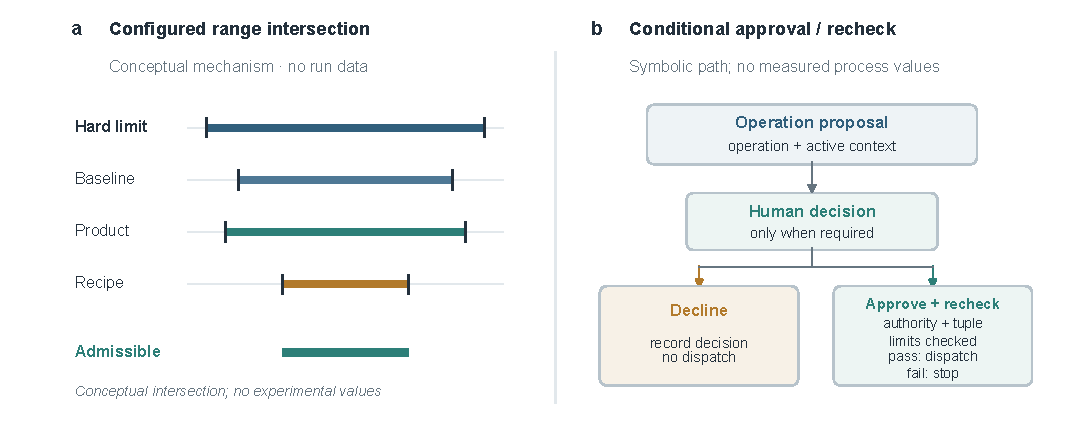
\includegraphics[width=\textwidth]{resources/fig5-nature-A.pdf}
\caption{Admission and approval boundaries. (a) Conceptual intersection of
the hard, baseline, product, and recipe bounds in Eq.~(\ref{eq:admission});
horizontal positions are schematic and encode no experimental values.
(b) When approval is required, a decline prevents dispatch; approval is
followed by authority, context, and limit rechecks.}
\label{fig:hitl}
\end{figure*}

A \texttt{recipe\_trial} illustrates the operation sequence: the handler
checks the bound recipe, active run, candidate parameters, and route timing;
if required, it requests approval; after revalidation, it submits a bounded
batch through the configured driver and returns a per-parameter receipt.
The caller can obtain later DAQ observations separately and may then update,
apply, or roll back a recipe. A trial neither saves nor applies a recipe
version. The driver registry maps semantic controls to configured protocol
drivers, keeping protocol details out of agent operation arguments.

At dispatch, the handler resolves the active production context, intersects
the applicable bounds, and applies route timing and approval requirements
before invoking the configured driver. The driver returns a graded receipt;
later acquisition samples are stored separately and linked to the operation
when the route provides matching context and timestamps. The evaluation uses
deterministic tool invocation and does not assess operator performance.

Receipts and observations answer different questions. A command result is
graded as readback-verified, transport-acknowledged, or unverified; a
readback mismatch can trigger up to three reads at 2\,s intervals. Recipe
batches retain per-parameter verification outcomes. A readback-verified result
records that the returned value matched the request; a transport acknowledgement
alone does not establish that the device applied it, and an unverified result
does not establish a matching readback. DAQ stores subsequent timestamped
process observations, while recipe history, approvals, and task records remain
with their owning services. Identifiers and timestamps can link these records
when available, but a later observation alone does not prove that the command
caused the measured change. Section~\ref{sec:eval} evaluates selected parts of
this evidence chain under the stated test conditions.
